\documentclass{beamer}
\usepackage[utf8]{inputenc}
\usepackage{amssymb}
\usepackage{amsthm}
\usepackage{amsmath}
\usepackage{tikz}
\usepackage{stmaryrd}

\title{Wide limits -- nonstandard analysis meets computational complexity}
\author{Ondra Ježil}

\usetheme{Boadilla}
\newcommand{\N}{\mathbb{N}}
\renewcommand{\P}{\mathcal{P}}
\newcommand{\Q}{\mathbb{Q}}
\newcommand{\R}{\mathbb{R}}
\newcommand{\M}{\mathcal{M}}
\newcommand{\A}{\mathcal{A}}
\newcommand{\B}{\mathcal{B}}
\newcommand{\I}{\mathcal{I}}
\newcommand{\st}{\text{st}}
\newcommand{\bbl}{\llbracket}
\newcommand{\bbr}{\rrbracket}
\newcommand{\G}{\mathcal{G}}
\newcommand{\0}{\textbf{0}}
\newcommand{\1}{\textbf{1}}
\newcommand{\abs}[1]{\lvert #1 \rvert}
\newcommand{\Th}{\text{Th}}
\newcommand{\EDGE}{\text{EDGE}}
\newcommand{\ALL}{\text{ALL}}
\newcommand{\nonEDGE}{\text{nonEDGE}}
\newcommand{\SK}{\text{SK}}
\newcommand{\CK}{\text{CK}}
\newtheorem{thrm}{Theorem}
\newtheorem{defi}{Definition}

\begin{document}

\frame{\titlepage}
\begin{frame}
\frametitle{Context}
\begin{itemize}[<+->] 
\item Imagine a ``growing'' sequence of finite structures, can we define a limit object (some kind of infinite structure)? (e.g. `a structure' = graph)
\item Yes! In many (sometimes overlapping) ways: arguments through compactness, ultraproduct, limits of dense graphs, graphons, \dots
\item Studying such structural limits can help us understand asymptotical behaviour of the growing sequence.
\item In this talk I will attempt to explain the central construction of my Master's thesis and present a few of my results. 
\item Key method -- Forcing
\end{itemize}
\end{frame}
\begin{frame}
\frametitle{An example}
\begin{itemize}[<+->] 
\item Consider $\varphi$ a first order $\varnothing$-sentence. 
\item e.g. $(\exists x)(\forall y)(x=y)$, $(\exists x)(\exists y)(x\not = y)$, $(\forall x)(\exists y)(\exists z)(\exists w)((x=y\leftrightarrow x\not = z) \land (w=y))$, \dots
\item For any set $S$ we can ask whether $S\models \varphi$. `Is the sentence $\varphi$ valid in $S$?'
\item \textbf{The problem:} Is $\{\abs{S}; S\models \varphi, S\text{ is finite} \}$ always finite or cofinite?
\end{itemize}
\end{frame}

\begin{frame}
\frametitle{Solution}
\begin{thrm}
Let $A:=\{\abs{S}; S\text{ is finite}, S\models \varphi\}$. Then either $A$ is finite or $\N\setminus A$ is finite.
\end{thrm}
\begin{proof}
Assume $A$ is not finite, we will prove, $\N\setminus A$ is infinite. 

For contradiction, assume $\N\setminus A$ is infinite. Compactness theorem from mathematical logic lets us then construct countable sets $S_1\models \varphi$ and $S_2\models \lnot \varphi$. But such sets without no structure are isomorphic! A contradiction.
\end{proof}
\end{frame}

\begin{frame}
\frametitle{Wide limits -- motivation}
\begin{itemize}[<+->] 
\item Our goal is similar. That is to understand asymptotical behaviour of a class of finite structures through one limiting object.
\item A key difference -- we have another parameter $F$, a set of functions with some restricted computational complexity. (e.g. polynomial time functions, function computed by decision trees, constant functions, \dots)
\item The wide limit $\lim_F \G_n$ represents how `an average' graph from $\G_k$ looks like to $F$. 
\end{itemize}
\vspace{1em}
\pause
\[\text{existential formulas in the limit}\leftrightarrow\text{hardness of search problems}\]
\end{frame}

\begin{frame}
\frametitle{Wide limits -- Setup}
\begin{itemize}[<+->] 
\item Let us now specify for what kind of classes of structures we will define a limit object for.
\item We restrict ourselves to graphs, but in theory any kind of relational (and even algebraic) structures can be used.
\end{itemize}
\pause
\begin{defi}[Wide sequence]
A sequence $\{\G_k\}_{k=1}^\infty$ of non-empty sets of finite graphs a \textbf{wide sequence} if
\begin{itemize}
\item there is a strictly increasing sequence of positive integers $\{g_k\}_{k=1}^\infty$ such that the vertex set of all $G\in\G_k$ is $\{0,\dots,g_k-1\}$,
\item $\lim_{k\to\infty}\abs{\G_k}=\infty$. (Hence, wide!)
\end{itemize}
\end{defi}
\end{frame}

\begin{frame}
\frametitle{Examples of wide sequences}
\begin{itemize}[<+->]
\item $\EDGE_k=\{(\{0,\dots,k-1\},E);\abs{E}=1\}$
\item $\nonEDGE_k=\{(\{0,\dots,k-1\},E);\abs{E}=\binom{k}{2}-1\}$
\item $\SK_k^{1/2}=\{(\{0,\dots,k-1\},E);E\text{ consist of exactly one $\lfloor\frac{k}{2} \rfloor$ clique}\}$
\item And so on...
\end{itemize}
\end{frame}

\begin{frame}
\frametitle{Nonstandard models of arithmetic -- definition}
\begin{itemize}[<+->]
\item Let us now introduce an important concept from mathematical logic which we will need later on.
\item By $\Th(\N)$ we mean the set of all true sentences of natural numbers. So axioms of ordered discrete semirings, all instances of induction, the four squares theorem, Fermat's last theorem and so on. 
\item In essence every theorem we will ever prove and more.
\item By standard theorems of model theory, there exist a semiring $\M\models \Th(\N)$ which is \textbf{not isomorphic} to $\N$.
\item $\M$ contains an isomorphic copy of $\N$ and then some `infinite numbers', we call those elements \textbf{nonstandard numbers}.
\item From now on we fix one $\M\models\Th(\N)$ which satisfies a technical condition. (It is $\aleph_1$-saturated.)
\end{itemize}
\end{frame}

\begin{frame}
\frametitle{Pseudofinite structures}
\begin{itemize}[<+->]
\item Let $n\in \M\setminus \N$ be a nonstandard number. We can then use it as an index in $\G_k$ to obtain the $n$-th level of $\{\G_k\}_{k=0}^\infty$. 
\item Graphs $G\in \G_n$ are what we call \textbf{pseudofinite}, they satisfy the theory of all finite graphs.
\item Example: In $\EDGE_n$ we get graphs on the infinite vertex set $\{0,\dots, n-1\}$ such that there is exactly one edge.
\end{itemize}
\end{frame}

\begin{frame}
\frametitle{The (random) vertex family $F$}

\begin{itemize}[<+->]
\item The other parameter of the limit yet to be specified is the family of functions $F$.
\item The main idea is this, imagine we uniformly sample a graph $\omega\in\G_n$, this would be impossible in a purely infinite setting, but we are in pseudofinite setting, so such sampling can take place in $\M$.
\item The sampled graph is then used as an input to the function $\alpha \in F$ and outputs an element in $\{0,\dots,g_k-1\}$ which is a vertex in each $\omega$.
\item The main vertex family we consider is $F_{rud}$ the family of functions computed by decision trees of depth $n^{1/t}$ for $t$ nonstandard.
\end{itemize}
\end{frame}

\begin{frame}
\frametitle{The vertex family $F_{rud}$}
\begin{defi}
The vertex family $F_{rud}$ consists of all functions $\alpha$ with input $\G_n$ and output computed by a directed tree of depth at most $g_n^{1/t}$, for some nonstandard $t$, whose form we present by the following example.
\begin{center}
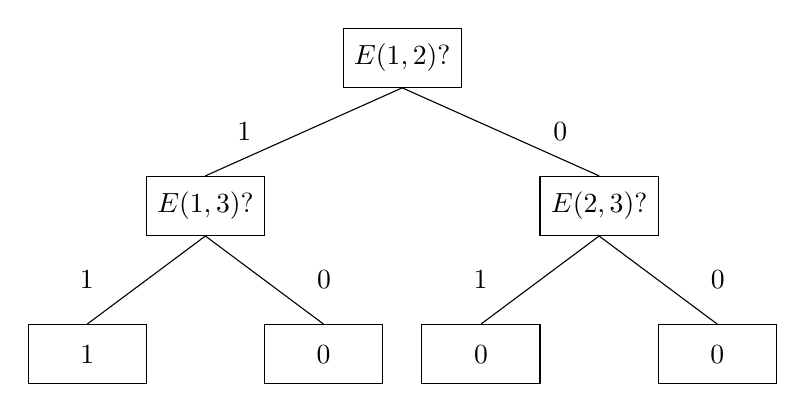
\begin{tikzpicture}[%
level 1/.style={sibling distance=5cm},
level 2/.style={sibling distance=3cm},
every node/.style = {draw, minimum width=1.5cm, minimum height=.75cm, anchor=north},
edge from parent path={(\tikzparentnode.south) -- (\tikzchildnode.north)}]
]
\node[] {$E(1,2)?$}
child { node[] {$E(1,3)?$}
    child { node[] {$1$} 
        edge from parent node[left,draw=none] {1}
	}
    child { node[] {$0$} 
        edge from parent node[right,draw=none] {0}
	}
    edge from parent node[left,draw=none] {1}
}
child { node[] {$E(2,3)?$} 
    child { node[] {$0$} 
    edge from parent node[left,draw=none] {1}
	}
    child { node[] {$0$} 
    edge from parent node[right,draw=none] {0}
	}
    edge from parent node[right,draw=none] {0}
};
\end{tikzpicture}
\end{center}
\end{defi}
\end{frame}

\begin{frame}
\frametitle{$\M$-rational numbers}

\begin{itemize}[<+->]
\item Let us elaborate on the uniform distrubution on $\Omega:=\G_k$.
\item We assign probability to sample each $\omega\in\M$ to be $1/\abs{\G_n}$ as an `$\M$-rational number'.
\item We can construct the $\M$-rational numbers $\Q^\M$ in an analogous way to how we construct $\Q$ from $\N$. (Add negative elements and take the fraction field.)
\item Those $\M$-rationals bounded by some $n\in\N$ we call \textbf{finite}, and those which are bounded by all $\frac{1}{n}$ we call \textbf{infinitesimal}.
\end{itemize}
\pause
\begin{thrm}
There exists a surjective, order preserving ring homomorphism $\varphi:\Q^\M_{fin}\to \R$ whose kernel is the ideal of infinitesimal numbers. We call the imagine $\st(q)$ the standard part of the $\M$-rational $q$.
\end{thrm}
\end{frame}

\begin{frame}
\frametitle{Nonstandard analysis}

How does this correspond to classical analysis?
\pause
\begin{thrm}
Let $\{b_k\}_{k=1}^\infty$ be a sequence of rational numbers then
\[\lim_{k\to\infty}b_k=r\in \R\]
if and only if for all nonstandard $n\in \M$
\[\st(b_n)=r\in \R.\]

\end{thrm}
\end{frame}

\begin{frame}
\frametitle{The Boolean algebra $\B$}
\begin{itemize}[<+->]
\item Boolean algebra is a complemented distributive lattice. The maximum element is denoted $\1$ and the minimum $\0$.
\item Examples $(\{0,1\},\land,\lor,\lnot,\0,\1),(\P(X),\cap,\cup,X\setminus -, \varnothing,X),\dots$
\item We start with the boolean algebra $\A=\{A\subseteq \G_n; A\in \M\}$ of subsets of the sample space $\G_n$ represented by elements in $\M$.
\item The counting measure is defined as $A\mapsto \abs{A}/\abs{\G_n}\in\Q^\M$.
\item The boolean algebra $\B$ is defined as the factor-algebra $\A/\I$ where $\I$ is the ideal of $\A$ of all elements with infinitesimal counting measure.
\end{itemize}
\end{frame}

\begin{frame}
\frametitle{The Boolean algebra $\B$ -- what we need}
\begin{itemize}[<+->]
\item \textbf{Key point}: The truth values of the first order sentences of the wide limit $\lim_{F}\G_n$ are the $\M$-definable subsets of $\G_n$ modulo sets of infinitesimal measure. We then have that $\B$ is a $\sigma$-algebra and that $\mu:A/\I \to \st(\abs{A}/\abs{\G_n})$ is measure in the classical sense.
\item Moreover, we have that $\B$ is a complete Boolean algebra, it contains all infinite disjunctions and conjunctions.
\end{itemize}
\end{frame}

\begin{frame}
\frametitle{The definition of a wide limit}
\begin{defi}[Wide limit]
For a wide sequence $\G_k$, vertex family $F$ and a nonstandard number $n$ we define the wide limit
\[\lim_F \G_n\]
as a $\B$-valued graph whose vertex set is $F$ and we interpret equality as
\[\lim_F\G_n\bbl\alpha = \beta \bbr=\{\omega \in \G_n; \alpha(\omega)=\beta(\omega) \}/\I,\]
and the edge relational symbol as
\[\lim_F\G_n\bbl E(\alpha,\beta) \bbr=\{\omega \in \G_n; E_\omega(\alpha(\omega),\beta(\omega)) \}/\I,\]
and let it commute with $\lnot$, $\land$, $\lor$ and interpret $\forall$ and $\exists$ respectively as infinite conjunctions and disjunctions.
\end{defi}
\end{frame}

\begin{frame}
\frametitle{$\G_k=\EDGE_k$}

\begin{itemize}[<+->]
\item Recall the wide sequence $\EDGE_k$ which roughly consist of all finite undirected graphs with one edge.
\item Every $\omega\in\EDGE_k$ has an edge.
\item What happens in the wide limit (with $F=F_{rud}$)?
\item What is
\[\lim_{F_{rud}}\EDGE_n\bbl(\exists x)(\exists y)E(x,y)\bbr=?\]
\pause
\item It is
\[\lim_{F_{rud}}\EDGE_n\bbl(\exists x)(\exists y)E(x,y)\bbr=\0\]
\end{itemize}


\end{frame}

\begin{frame}
\begin{thrm}
\[\lim_{F_{rud}}\EDGE_n\bbl(\exists x)(\exists y)E(x,y)\bbr=\0\]
\end{thrm}
\begin{proof}\renewcommand{\qedsymbol}{}
The universe of the wide limit is $F_{rud}$ the (random) vertices computed by decision trees of depth $n^{1/t}=g_n^{1/t}$ for some $t>\N$.

So we need to prove that any two such trees find the edge in uniformly smapled $\omega\in\EDGE_n$ with uniform probability. We can just compose the trees into one tree $T$ which actually outputs the edge.
\end{proof}
\end{frame}

\begin{frame}
\begin{thrm}
\[\lim_{F_{rud}}\EDGE_n\bbl(\exists x)(\exists y)E(x,y)\bbr=\0\]
\end{thrm}
\begin{proof}[Proof cont.]\renewcommand{\qedsymbol}{}
So assume $T$ is a possibly successful tree. We will prove it is definitely not successful.

Go down the tree and answer $\textbf{0}$ to every query of the tree. Then the $T$ cannot possibly succeed, what is the ratio of $\omega\in\EDGE_k$ which result in such answers? 

\end{proof}
\end{frame}

\begin{frame}
\begin{thrm}
\[\lim_{F_{rud}}\EDGE_n\bbl(\exists x)(\exists y)E(x,y)\bbr=\0\]
\end{thrm}
\begin{proof}[Proof cont.]
So we compute the ratio of those graphs in which the edge in not among $n^{1/t}$ many specified pairs of vertices.

\vspace{-1em}
\begin{align}
\frac{\binom{n-n^{1/t}}{2}}{\binom{n}{2}}&=\frac{(n-n^{1/t})(n-n^{1/t}-1)}{n(n-1)}\\
&=\left(1-\frac{n^{1/t}}{n}\right)\left(1-\frac{n^{1/t}+1}{n-1}\right)\\
&\geq 1-\frac{2n^{1/t}+2}{n-1}
\end{align}
but the standard part of (3) is $1$! So the probability any tree succeeds is infinitesimally close to $0$.
\end{proof}
\end{frame}

\begin{frame}
\frametitle{Too sparse wide sequences}
\begin{itemize}[<+->]
\item We say a wide sequence $\G_k$ is too sparse, if its wide limit is the empty graph.
\item We can analyze this situation more generally for $F_{rud}$.
\end{itemize}
\pause
\begin{thrm}
If the probability that a uniformly random pair of vertices on a uniformly random $G\in\G_k$ is $o(1/\sqrt[j]{k})$ for any $j\in \N$ then
\[\lim_{F_{rud}}\G_n\bbl(\exists x)(\exists y)E(x,y)\bbr=\0.\]
\end{thrm}
\end{frame}

\begin{frame}
\frametitle{$\G_k=\ALL_k$}
\begin{itemize}[<+->]
\item No edges? Too boring! \pause
\item Let us see some stuff! \pause
\item Consider $\ALL_k$ the wide sequence of all finite graphs, there ought to be something, right?
\end{itemize}
\pause
\begin{thrm}[Everything exists]
Let $\varphi(\overline x)$ be a formula in the langauge of graphs (possibly with parameters), then
\[\lim_{F_{rud}}\ALL_k\bbl(\exists \overline x)\varphi(x)\bbr=\1.\]
\end{thrm}
\begin{proof}[Proof. (sketch)]
Iterate search on $n^{1/t}$ different tuples of $\omega$ and use mutual independence.
\end{proof}
\end{frame}

\begin{frame}
\frametitle{Large clique}
\begin{itemize}
\item Let $\SK_k^{1/2}$ be the wide sequence of all graphs containing one copy of a $\lfloor k/2\rfloor$-clique.
\end{itemize}
\pause
\begin{thrm}
\[\lim_{F_{rud}}^{G_{rud}}\G_n\bbl\text{there is a $\lfloor n/(2\ln n) \rfloor$ clique}\bbr=\1\]
\end{thrm}
\pause
\begin{itemize}
\item Open problem: Is this the biggest clique here? What about in the wide sequence which contains a large clique and possibly other edges?
\end{itemize}
\end{frame}

\begin{frame}
\frametitle{What's next?}
\begin{itemize}[<+->]
\item Further analyze when we get the truth values strictly in the set $\{\0,\1\}$.
\item Analyze the $F_{poly}$, connection to $\textbf{P}$ vs. $\textbf{NP}$.
\item Easily generalizable to any relational and algebraic structure.
\item One can then take a wide limit of $\textbf{CSP}(\mathbb{A})$, connection to tractability.
\item The ultimate direction to pursue is to characterize some wide limit independently of the direct definition -- this immediatelly results in (probabilistic) lower and upper bounds for $F$.
\end{itemize}
\end{frame}

\begin{frame}
\begin{center}
\Huge
\[\lim_{F}\G_n\bbl\textbf{Thank you!}\bbr=\1\]
\end{center}
\end{frame}

\end{document}
